\documentclass[14pt]{extbook}
\usepackage{multicol, enumerate, enumitem, hyperref, color, soul, setspace, parskip, fancyhdr} %General Packages
\usepackage{amssymb, amsthm, amsmath, latexsym, units, mathtools} %Math Packages
\everymath{\displaystyle} %All math in Display Style
% Packages with additional options
\usepackage[headsep=0.5cm,headheight=12pt, left=1 in,right= 1 in,top= 1 in,bottom= 1 in]{geometry}
\usepackage[usenames,dvipsnames]{xcolor}
\usepackage{dashrule}  % Package to use the command below to create lines between items
\newcommand{\litem}[1]{\item#1\hspace*{-1cm}\rule{\textwidth}{0.4pt}}
\pagestyle{fancy}
\lhead{Progress Quiz 7}
\chead{}
\rhead{Version B}
\lfoot{6523-2736}
\cfoot{}
\rfoot{test}
\begin{document}

\begin{enumerate}
\litem{
Solve the quadratic equation below. Then, choose the intervals that the solutions belong to, with $x_1 \leq x_2$ (if they exist).\[ 16x^{2} +9 x -2 = 0 \]\begin{enumerate}[label=\Alph*.]
\item \( x_1 \in [-12.14, -11.48] \text{ and } x_2 \in [1.89, 2.9] \)
\item \( x_1 \in [-15.12, -14.66] \text{ and } x_2 \in [13.8, 14.86] \)
\item \( x_1 \in [-0.45, -0.04] \text{ and } x_2 \in [0.66, 1.27] \)
\item \( x_1 \in [-1.27, -0.24] \text{ and } x_2 \in [0.01, 0.49] \)
\item \( \text{There are no Real solutions.} \)

\end{enumerate} }
\litem{
Solve the quadratic equation below. Then, choose the intervals that the solutions belong to, with $x_1 \leq x_2$ (if they exist).\[ 14x^{2} -15 x -2 = 0 \]\begin{enumerate}[label=\Alph*.]
\item \( x_1 \in [-18.39, -17.58] \text{ and } x_2 \in [18.87, 19.46] \)
\item \( x_1 \in [-1.48, -1.08] \text{ and } x_2 \in [-0.9, 0.56] \)
\item \( x_1 \in [-0.7, 0.98] \text{ and } x_2 \in [0.54, 1.44] \)
\item \( x_1 \in [-2.36, -1.65] \text{ and } x_2 \in [16.54, 17.21] \)
\item \( \text{There are no Real solutions.} \)

\end{enumerate} }
\litem{
Solve the quadratic equation below. Then, choose the intervals that the solutions $x_1$ and $x_2$ belong to, with $x_1 \leq x_2$.\[ 25x^{2} -50 x + 24 = 0 \]\begin{enumerate}[label=\Alph*.]
\item \( x_1 \in [0.43, 0.63] \text{ and } x_2 \in [1.59, 1.76] \)
\item \( x_1 \in [0.23, 0.31] \text{ and } x_2 \in [3.93, 4.11] \)
\item \( x_1 \in [0.77, 0.84] \text{ and } x_2 \in [0.86, 1.45] \)
\item \( x_1 \in [0.31, 0.49] \text{ and } x_2 \in [2.16, 2.56] \)
\item \( x_1 \in [19.91, 20.29] \text{ and } x_2 \in [29.96, 30.41] \)

\end{enumerate} }
\litem{
Graph the equation below.\[ f(x) = (x+4)^2 + 19 \]\begin{enumerate}[label=\Alph*.]
\begin{multicols}{2}\item 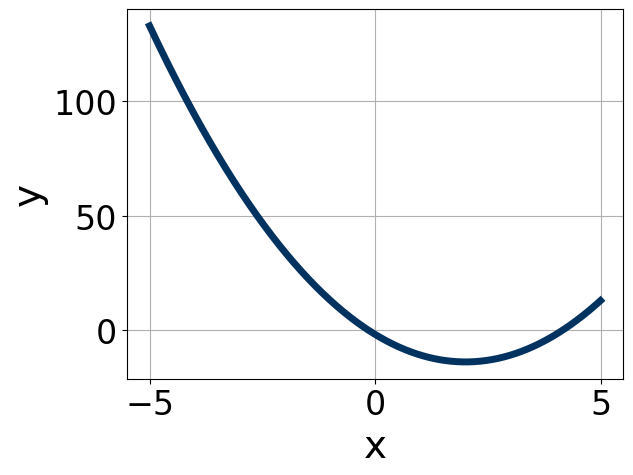
\includegraphics[width = 0.3\textwidth]{../Figures/quadraticEquationToGraphAB.png}\item 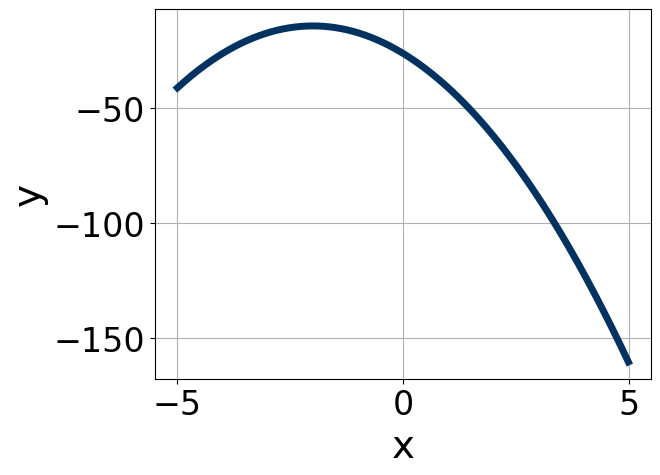
\includegraphics[width = 0.3\textwidth]{../Figures/quadraticEquationToGraphBB.png}\item 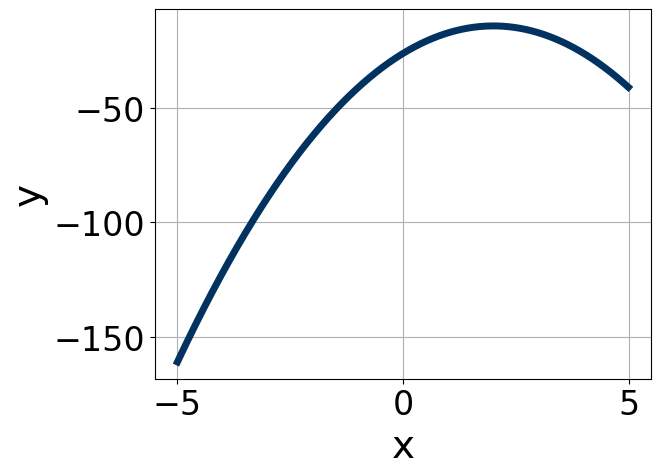
\includegraphics[width = 0.3\textwidth]{../Figures/quadraticEquationToGraphCB.png}\item 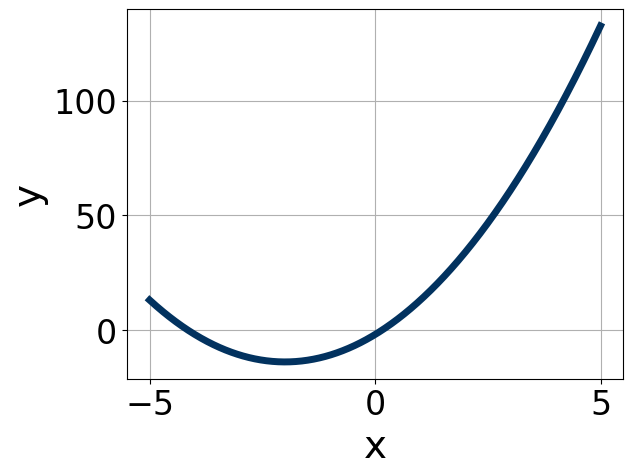
\includegraphics[width = 0.3\textwidth]{../Figures/quadraticEquationToGraphDB.png}\end{multicols}\item None of the above.
\end{enumerate} }
\litem{
Factor the quadratic below. Then, choose the intervals that contain the constants in the form $(ax+b)(cx+d); b \leq d.$\[ 54x^{2} -33 x -10 \]\begin{enumerate}[label=\Alph*.]
\item \( a \in [2, 5], \hspace*{5mm} b \in [-5, 0], \hspace*{5mm} c \in [17.94, 18.63], \text{ and } \hspace*{5mm} d \in [-4, 11] \)
\item \( a \in [0, 2], \hspace*{5mm} b \in [-47, -43], \hspace*{5mm} c \in [0.25, 1.76], \text{ and } \hspace*{5mm} d \in [6, 14] \)
\item \( a \in [10, 21], \hspace*{5mm} b \in [-5, 0], \hspace*{5mm} c \in [2.33, 3.28], \text{ and } \hspace*{5mm} d \in [-4, 11] \)
\item \( a \in [5, 9], \hspace*{5mm} b \in [-5, 0], \hspace*{5mm} c \in [8.1, 9.59], \text{ and } \hspace*{5mm} d \in [-4, 11] \)
\item \( \text{None of the above.} \)

\end{enumerate} }
\litem{
Factor the quadratic below. Then, choose the intervals that contain the constants in the form $(ax+b)(cx+d); b \leq d.$\[ 36x^{2} +60 x + 25 \]\begin{enumerate}[label=\Alph*.]
\item \( a \in [0.32, 1.87], \hspace*{5mm} b \in [25, 38], \hspace*{5mm} c \in [0.57, 1.55], \text{ and } \hspace*{5mm} d \in [28, 35] \)
\item \( a \in [1.35, 3.14], \hspace*{5mm} b \in [1, 10], \hspace*{5mm} c \in [17.02, 20.02], \text{ and } \hspace*{5mm} d \in [3, 6] \)
\item \( a \in [16.04, 18.73], \hspace*{5mm} b \in [1, 10], \hspace*{5mm} c \in [1.19, 2.49], \text{ and } \hspace*{5mm} d \in [3, 6] \)
\item \( a \in [5.34, 6.94], \hspace*{5mm} b \in [1, 10], \hspace*{5mm} c \in [5.69, 7.04], \text{ and } \hspace*{5mm} d \in [3, 6] \)
\item \( \text{None of the above.} \)

\end{enumerate} }
\litem{
Graph the equation below.\[ f(x) = -(x-2)^2 + 11 \]\begin{enumerate}[label=\Alph*.]
\begin{multicols}{2}\item 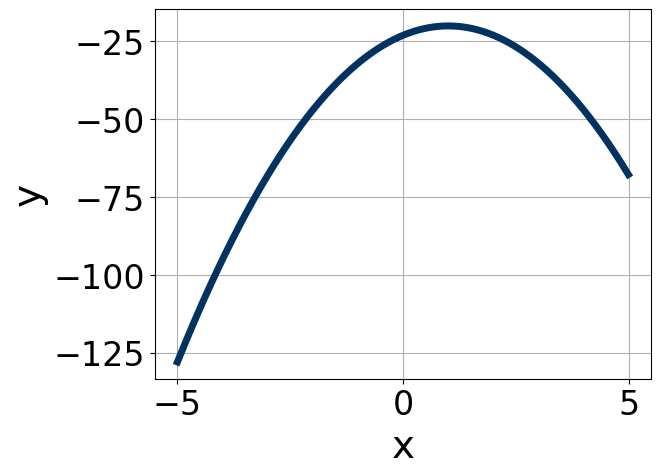
\includegraphics[width = 0.3\textwidth]{../Figures/quadraticEquationToGraphCopyAB.png}\item 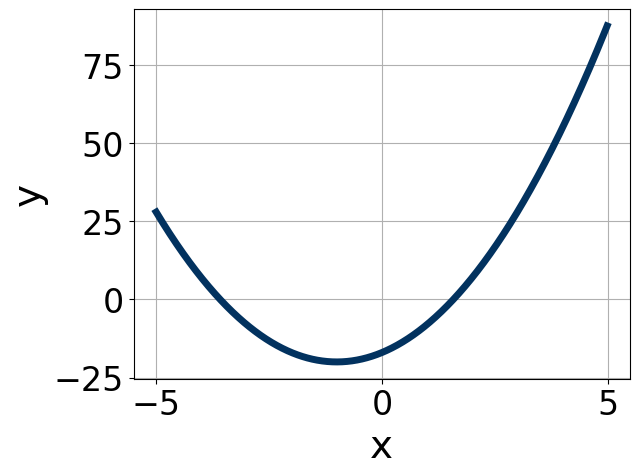
\includegraphics[width = 0.3\textwidth]{../Figures/quadraticEquationToGraphCopyBB.png}\item 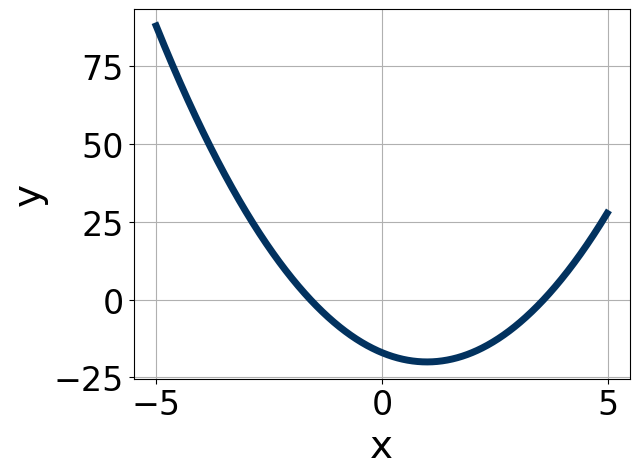
\includegraphics[width = 0.3\textwidth]{../Figures/quadraticEquationToGraphCopyCB.png}\item 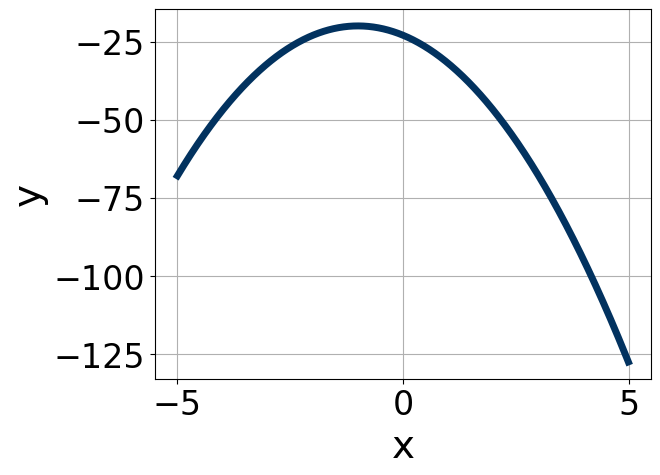
\includegraphics[width = 0.3\textwidth]{../Figures/quadraticEquationToGraphCopyDB.png}\end{multicols}\item None of the above.
\end{enumerate} }
\litem{
Solve the quadratic equation below. Then, choose the intervals that the solutions $x_1$ and $x_2$ belong to, with $x_1 \leq x_2$.\[ 15x^{2} +2 x -24 = 0 \]\begin{enumerate}[label=\Alph*.]
\item \( x_1 \in [-1.74, -0.68] \text{ and } x_2 \in [1.09, 1.24] \)
\item \( x_1 \in [-3.66, -1.59] \text{ and } x_2 \in [0.57, 0.6] \)
\item \( x_1 \in [-1.12, -0.55] \text{ and } x_2 \in [2.35, 2.48] \)
\item \( x_1 \in [-6.32, -2.89] \text{ and } x_2 \in [0.3, 0.51] \)
\item \( x_1 \in [-21.35, -19.97] \text{ and } x_2 \in [17.92, 18.32] \)

\end{enumerate} }
\litem{
Write the equation of the graph presented below in the form $f(x)=ax^2+bx+c$, assuming  $a=1$ or $a=-1$. Then, choose the intervals that $a, b,$ and $c$ belong to.
\begin{center}
    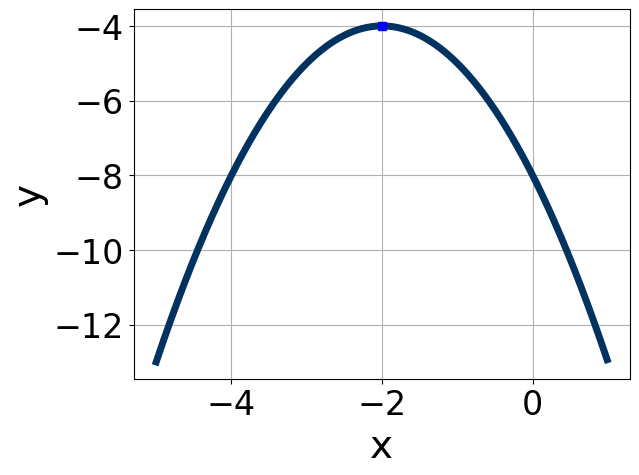
\includegraphics[width=0.5\textwidth]{../Figures/quadraticGraphToEquationCopyB.png}
\end{center}
\begin{enumerate}[label=\Alph*.]
\item \( a \in [0, 2], \hspace*{5mm} b \in [-10, -7], \text{ and } \hspace*{5mm} c \in [17, 21] \)
\item \( a \in [-1, 0], \hspace*{5mm} b \in [-10, -7], \text{ and } \hspace*{5mm} c \in [-12, -10] \)
\item \( a \in [0, 2], \hspace*{5mm} b \in [4, 9], \text{ and } \hspace*{5mm} c \in [17, 21] \)
\item \( a \in [0, 2], \hspace*{5mm} b \in [-10, -7], \text{ and } \hspace*{5mm} c \in [8, 14] \)
\item \( a \in [-1, 0], \hspace*{5mm} b \in [4, 9], \text{ and } \hspace*{5mm} c \in [-12, -10] \)

\end{enumerate} }
\litem{
Write the equation of the graph presented below in the form $f(x)=ax^2+bx+c$, assuming  $a=1$ or $a=-1$. Then, choose the intervals that $a, b,$ and $c$ belong to.
\begin{center}
    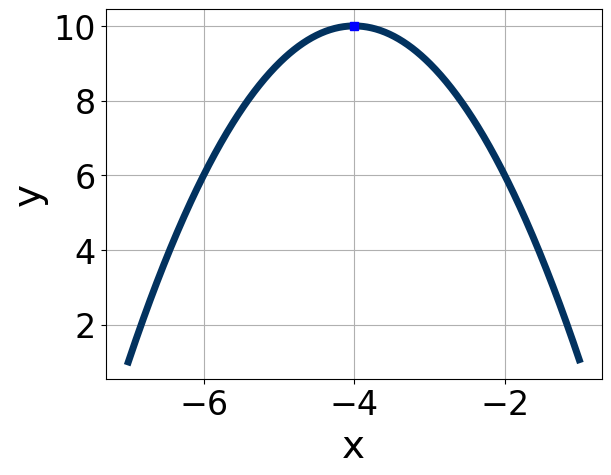
\includegraphics[width=0.5\textwidth]{../Figures/quadraticGraphToEquationB.png}
\end{center}
\begin{enumerate}[label=\Alph*.]
\item \( a \in [0.1, 2.2], \hspace*{5mm} b \in [5, 9], \text{ and } \hspace*{5mm} c \in [18, 22] \)
\item \( a \in [-1.6, -0.9], \hspace*{5mm} b \in [-11, -6], \text{ and } \hspace*{5mm} c \in [-22, -14] \)
\item \( a \in [0.1, 2.2], \hspace*{5mm} b \in [-11, -6], \text{ and } \hspace*{5mm} c \in [18, 22] \)
\item \( a \in [-1.6, -0.9], \hspace*{5mm} b \in [5, 9], \text{ and } \hspace*{5mm} c \in [-13, -9] \)
\item \( a \in [-1.6, -0.9], \hspace*{5mm} b \in [-11, -6], \text{ and } \hspace*{5mm} c \in [-13, -9] \)

\end{enumerate} }
\end{enumerate}

\end{document}